\chapter{Resultat}
\label{cha:results}

\section{Systembeskrivning - gammal}
%% Översiktlig beskrivning system, dokument
%% Vad har kunden för värde hos det som skapats?

Systemet består hårdvarumässigt av ett rotationsbord, en avståndskamera och en linjärenhet för att flytta avståndskameran längs en axel. För att styra detta fanns det sedan tidigare mjukvara som kan utföra en enskild skanning. Detta projekt har resulterat i mjukvara för att utföra fler skanningar från olika vinklar och sammanfoga dessa till ett komplett objekt som kan skrivas ut på en 3D-skrivare. Resultatet av projektet består av en mjukvara som kan användas för att skanna ett fysiskt objekt och skriva ut en kopia av objektet på en 3D-skrivare.

I nuläget finns en väl genomtänkt plan för hur projektet ska genomföras och hur systemet ska fungera. Det finns en projektplan som beskriver hur utvecklingsarbetet ska gå till och en kravspecifikation som säger vad systemet måste uppfylla för att bli godkänt av kunden.

Det har även tagits fram en arkitekturbeskrivning som förklarar hur systemet ska fungera och vilka moduler som ska finnas. Arkitekturen ger en bra utgångspunkt för hur systemet ska implementeras. I arkitekturbeskrivningen finns det förklarat vilka noder systemet ska bestå av och hur de ska kommunicera med varandra. Det underlättar under utvecklingen då varje nod har tydligt definierad in- och utdata och det är tydligt specificerat vad noden ska utföra. Det är möjligt att ändringar kommer att göras i arkitekturen längre fram i projektet men troligen kommer inga större förändringar att behövas.

Arkitekturen är uppbyggd i ROS vilket innebär att de flesta noder i systemet fungerar som en service som tar emot en request för att utföra någonting och när den är klar svarar den med en response. Detta gör att alla noder har tydliga gränssnitt mellan varandra vilket resulterar i en bra separation mellan olika moduler.

Noden för att wrappa TreeDs kommandoradsgränssnitt för att utföra enskilda skanningar är färdigimplementerad och testad. Den kan användas av det övriga systemet genom att kalla på en service i ROS och ange vilka vinklar man vill ha en skanning från. TreeD-wrapper-noden utför då skanningen och returnerar det enskilda punktmolnet.

Systemet kan även samla in fler punktmoln. Detta görs av punktmolnsnoden som tar in ett värde för hur noggrant objektet ska skannas. Sedan utförs ett antal skanningar genom att TreeD-wrappern kallas. Nästa steg är att dessa inkompletta punktmoln ska registreras till ett punktmoln för hela objektet men det är inte implementerat än. Trots att punktmolnen inte registreras i nuläget finns det ett värde för kunden att kunna utföra fler skanningar.

Mycket tid under den första iterationen av projektet har lagts på att utforska och undersöka olika tekniker och algoritmer. Som resultat av det finns det mycket nyttig kunskap i projektgruppen och även en del testkod för att utföra olika delar. Testkoden kommer till stor del kunna användas som utgångspunkt för det riktiga systemet.

\section{Systembeskrivning - ny}
\subsection{Kommandoradsgränssnitt (CLI)}

Systemet kan kontrolleras av ett CLI som kan ta in olika parametrar för att anpassa registreringen. Det finns även alternativ för att bara registrera eller bara mesha objekt. När man kör programmet med hjälp av kommandoradsgränssnittet väljer man vilka filer eller mappar med filer programmet ska läsa in och använda. Hur de används beror på alternativen. Ett exempel på ett anrop är:\\\\
\textit{3DCopy -v --max-corr-dist 15 path/to/register/ output}\\\\
Det anropet kommer registrera och sedan mesha .pcd filerna i mappen path/to/register/ och döpa det kompletta punktmolnet respektive färdiga meshen till output.pcd och output.stl. Under registreringen och meshningen kommer programmet att skriva ut information om processen på grund av -v flaggan som står för \textit{verbose mode}. Om man undrar vilka alternativ som finns kan man använda -h flaggan så skriver programmet ut vilka alternativ som finns och hur man använder programmet med hjälp av kommandoradsgränssnittet. 

\subsection{GUI}
För att lättare kunna styra mjukvaran utvecklades också ett GUI. GUI:t har nästintill samma funktionalitet som CLI:t och målet med att ha samma funktionalitet är att det inte ska spela någon roll om man använder CLI eller GUI.

\begin{figure}[H]
	\centering
	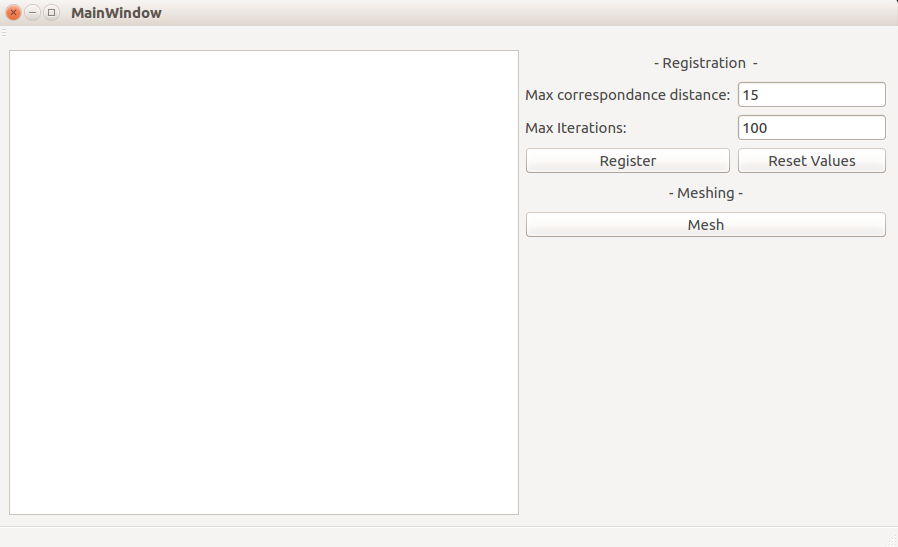
\includegraphics[width=130mm]{figures/3DCopyGUI.PNG}
	\caption{GUI:t för 3DCopy i slutet av iteration 2.}
	\label{fig:3dcopy_gui}
\end{figure}

De funktioner som finns i GUI:t just nu är Register som öppnar en dialog där man får välja en mapp som innehåller de punktmoln som man vill registrera. Det finns också en Mesh funktion där en dialog öppnas och man får välja det punktmoln som man vill mesha. Det finns också en funktion för att återställa parametervärdena för registreringen, Reset Values.

\section{Gemensamma erfarenheter}
%% Goda, mindre bra
%% I projektets alla faser
%% Tekniska, process-relaterade

I detta avsnitt presenteras de erfarenheter som gruppen har samlat på sig under projektets gång.

\subsection{Övergripande projekterfarenheter}

Att göra efterforskningar innan man börjar med någonting är väldigt viktigt och det märktes direkt i projektets början. Både genom att större delen av våra efterforskningar kom till stor hjälp direkt i projektet och bara några dagar in i första iterationen märktes det att det fanns några områden vi behövde läsa på mer om innan vi kunde skriva kod. Ett exempel på bra efterforskning som gjordes i förstudien var efterforskningarna kring ROS där alla gruppmedlemmar gick igenom tutorials och läste dokumentation som utvecklingsledaren gått igenom och tagit fram. I slutet av förstudien gjordes en gemensam kodutmaning där alla fick skriva varsin chattklient med hjälp av ROS. Kodutmaningen ledde till att alla kom in i ROS, Git, Python och andra verktyg som skulle användas under resten av projektet.


\subsection{Erfarenheter gällande kommunikation}

Betydelsen av kommunikation var stor under projektets gång. Verktygen Slack och Trello har använts flitigt och varit givande för gruppen. Med Slack har vi alltid kunnat nå varandra snabbt och smidigt. Vi har kunnat hålla informationsflöden skilda och sorterade i olika kanaler. Funktioner som påminnelser och trådar har också varit till stor hjälp för att lätt kunna komma åt den informationen som man vill åt i flödena. För att ha en översikt i hur det går med olika delar av projektet har man använt Trello. Genom att ha olika listor för statusen av dokument och funktioner under utveckling har gjort att man som gruppmedlem lätt kunnat se hur det går och vad man behöver göra. 


\subsection{Erfarenheter gällande kvalité}

Kvalité har varit viktigt för gruppen och kvalitetsansvarig har gjort ett bra jobb med att se till att projektets kod och dokument håller en hög standard. Detta framförallt genom granskning av dokument och kod. All kod i projektet har genomgått granskning för att säkerställa god kvalité. Till detta har Githubs pull request-funktion använts där alla gruppmedlemmar kunnat kommentera och diskutera koden innan den går in i master branchen hos repositoriet. Dokumenten har också granskats, då genom korrekturläsning. All denna granskning har varit mycket bra för att se hur andra skriver dokument och kod.

\subsection{Erfarenheter av att bygga vidare på ett projekt}

I mitten av projektet upptäckte gruppen att det system som skulle vidareutvecklas inte fungerade tillräckligt stabilt för att det skulle vara möjligt att integrera med det system som gruppen utvecklade. Gruppen litade på att kunden hade god insikt i det tidigare systemet och eftersom att dessa fel inte togs upp i början av projektet förutsatte gruppen att det tidigare systemet inte innehöll några fel.

Eftersom att gruppen inte hade någon anledning qtt tro att det tidigare systemet innehöll fel så genomfördes ingen testning av det tidigare systemet. Det saknades också testdokumentation från den grupp som hade utvecklat det tidigare systemet. Det visar vikten av att väl dokumentera sitt system för att undvika problem i framtiden.


\section{Översikt över individuella bidrag}

Här listas de individuella bidrag som gruppens medlemmar har bidragit med till rapporten:

\begin{itemize}
	\item Dunström, Hampus - Hur påverkas ett team av sin arbetsmiljö?
	\item Holmberg, Olof - Kontexters påverkan vid testning av GUI
	\item Jannering, Gustav - Hur kravhanteringsmetoder påverkar ett utvecklingsprojekt
	\item Karlsson, Michael - Analys av punktmolnsregistrering
	\item Lundberg, Martin - Att bygga ett system i ROS
	\item Tuhkala, Hannes - Att använda sig av LaTeX för större dokument
	\item Wallström, Fredrik - Kvalitetsarbete i praktiken
\end{itemize}


%%%%%%%%%%%%%%%%%%%%%%%%%%%%%%%%%%%%%%%%%%%%%%%%%%%%%%%%%%%%%%%%%%%%%%
%%% results.tex ends here